\chapter{Implementación}

\textbf{Plataforma de desarrollo}

Para construir el sistema se eligió Chatfuel \cite{sarinho2017splimbo} como herramienta de desarrollo. Esta herramienta está basada en bloques de contenido. Un bloque puede tener varios contenidos o tarjetas:
\begin{itemize}
\item Texto
\item Imágen
\item Galería de imágenes
\item Respuestas rápidas
\item Plugins:
\begin{itemize}
	\item API JSON, entrada de texto del usuario, crear variables de usuario, ir a bloque, Zapier, entre otras.
\end{itemize}
\end{itemize}

Las ventajas que esta plataforma ofrece son varias:
\begin{itemize}
\item Creación gráfica de bloques de contenido
\item Creación de la lógica entre bloques
\item Publicación automática a Facebook
\item Portabilidad a otras plataformas (Facebook Messenger, Telegram y próximamente Whatsapp, Kik y Slack)
\item Integración con plataformas de análisis
\end{itemize}

\textbf{Bloques de contenido}
A partir del uso de esta herramienta se construyeron los bloques de contenido. Los bloques se dividen en varias categorías:
Default - Aquí se define el saludo de bienvenida y la respuesta por defecto cuando la entrada de texto no se reconoce

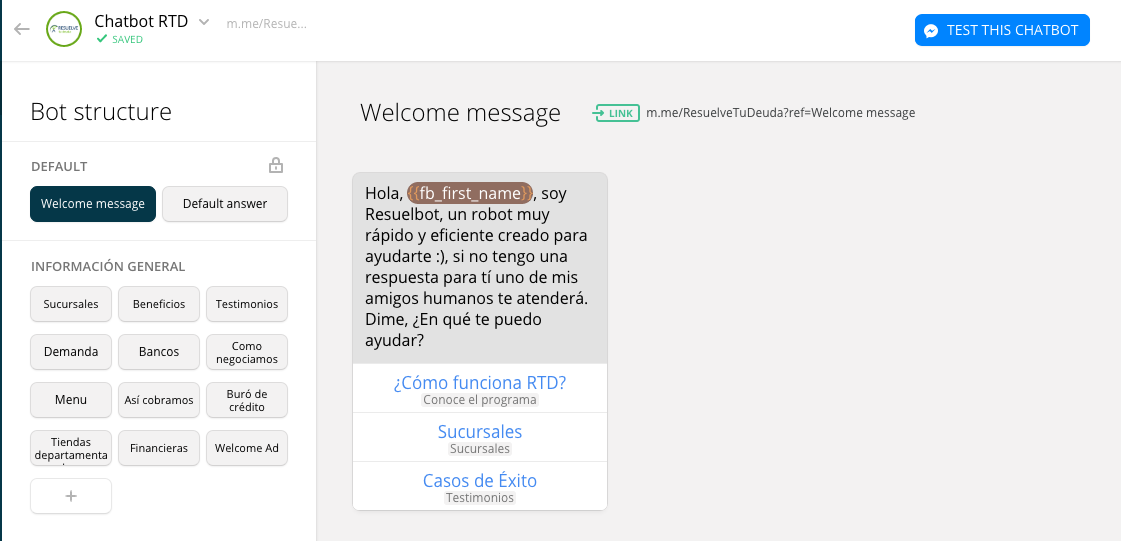
\includegraphics[width=\textwidth]{chatfuelWelcome.jpg}

Información General -  Aquí se da información de la empresa como sucursales, beneficios y testimonios; para aumentar la confianza del cliente sobre la reparadora de crédito.

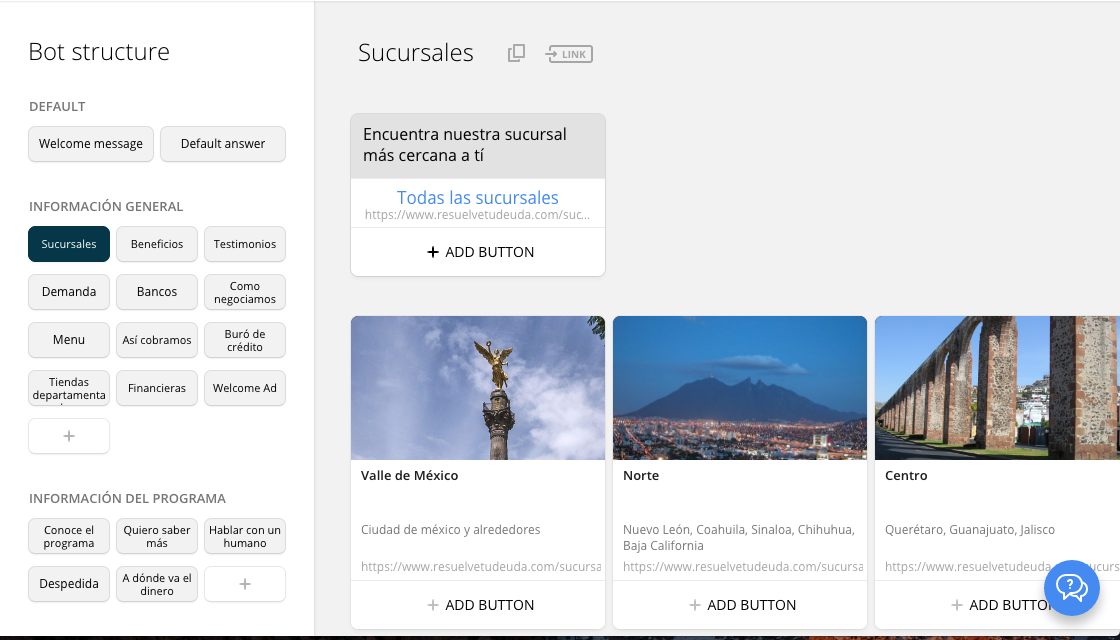
\includegraphics[width=\textwidth]{chatfuelSucursales.jpg}

Información del programa - Información general para conocer el programa de reparación de crédito

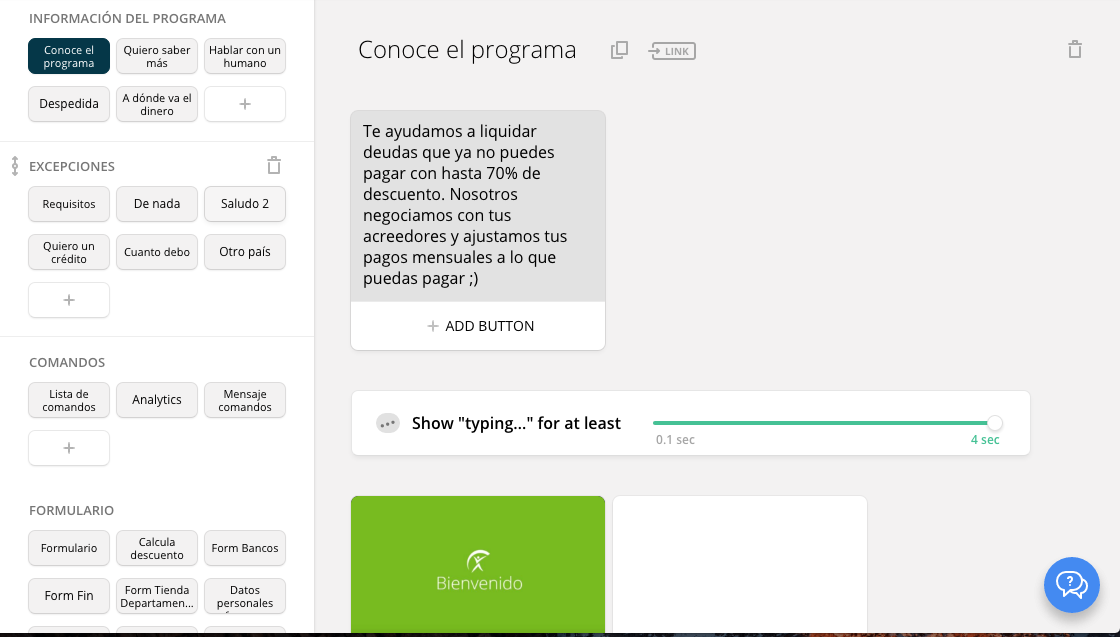
\includegraphics[width=\textwidth]{chatfuelConoceElPrograma.jpg}

Excepciones - Para algunos flujos, como el de cotización de descuento, existen requisitos (mínimo \$35,000 de deuda acumulada, ciertos bancos, etc). Si no se cubren los requisitos se muestra una excepción general de ese flujo explicando los requerimientos mínimos.

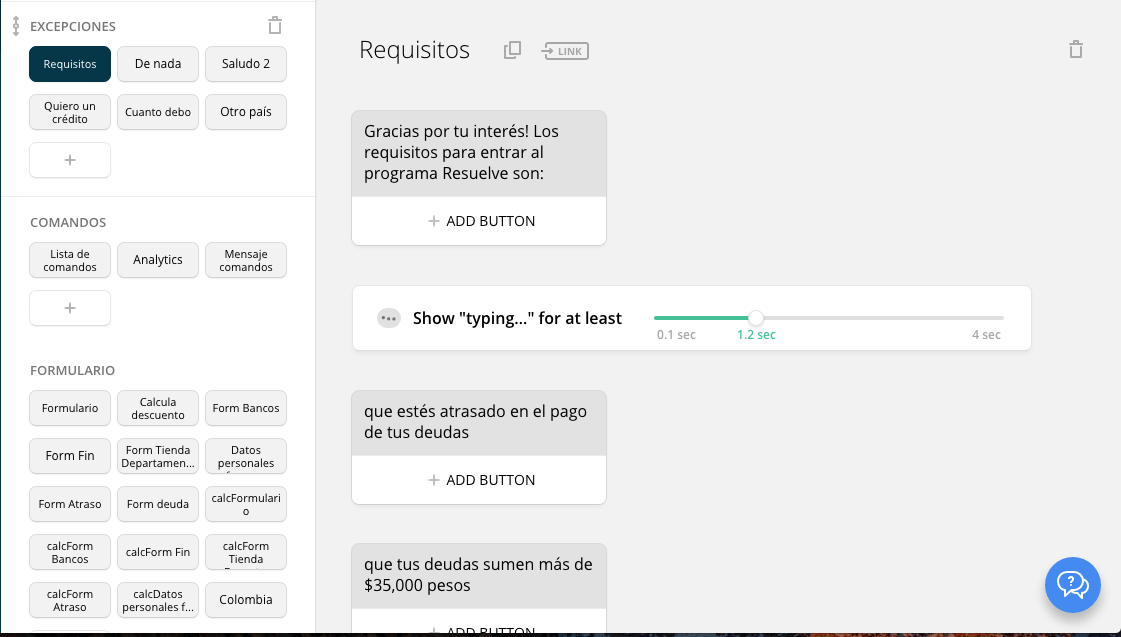
\includegraphics[width=\textwidth]{chatfuelRequisitosExep.jpg}

Comandos - La intención de este bloque es dar a conocer las funcionalidades que no son evidentes en la conversación y los detonadores que inician diferentes tipos de conversaciones.

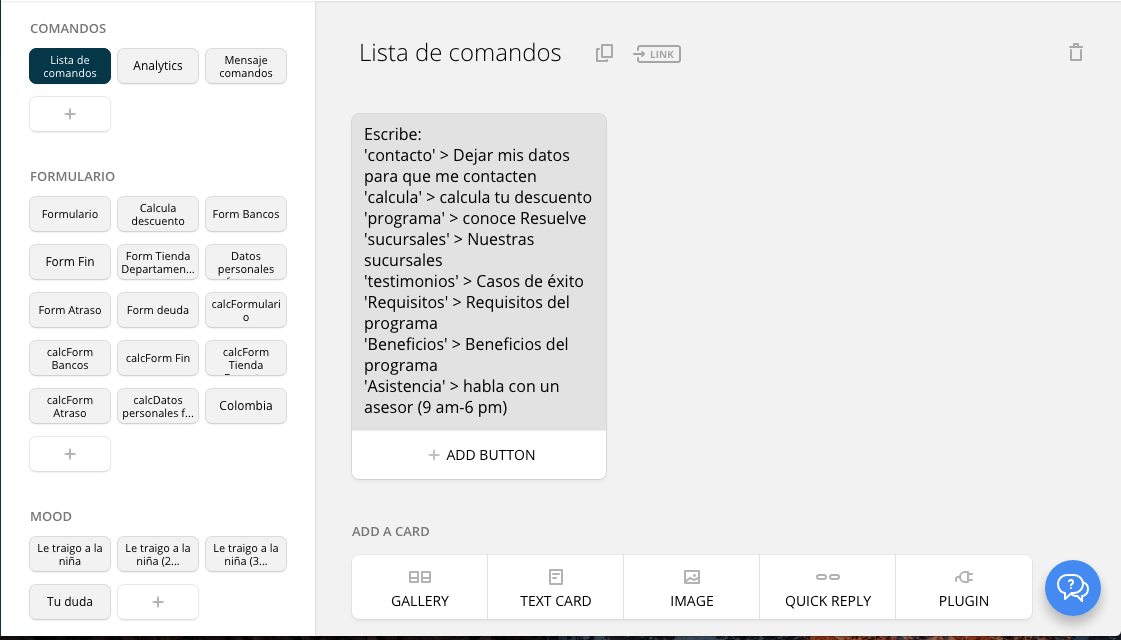
\includegraphics[width=\textwidth]{chatfuelComandos.jpg}

Anuncios de Facebook - Uno de los canales que más tráfico atrae es el de anuncios pagados en Facebook. Para poder medir el impacto de las campañas utilizadas se crearon el mismo número de bloques como campañas. En estos bloques se instancia el valor de la campaña de la que viene el usuario y se envía al final junto con los datos de contacto, si resulta en un lead, a la base de datos.

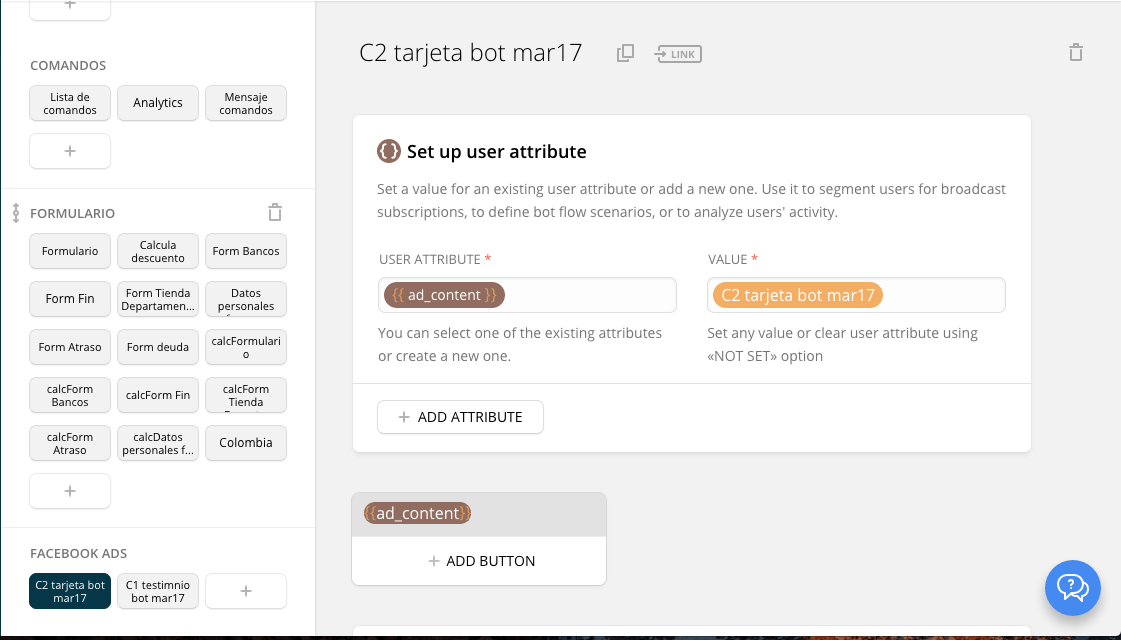
\includegraphics[width=\textwidth]{chatfuelFBAds.jpg}

Formulario - En esta sección está todo el proceso de captación de datos de contacto del usuario interesado en el producto.

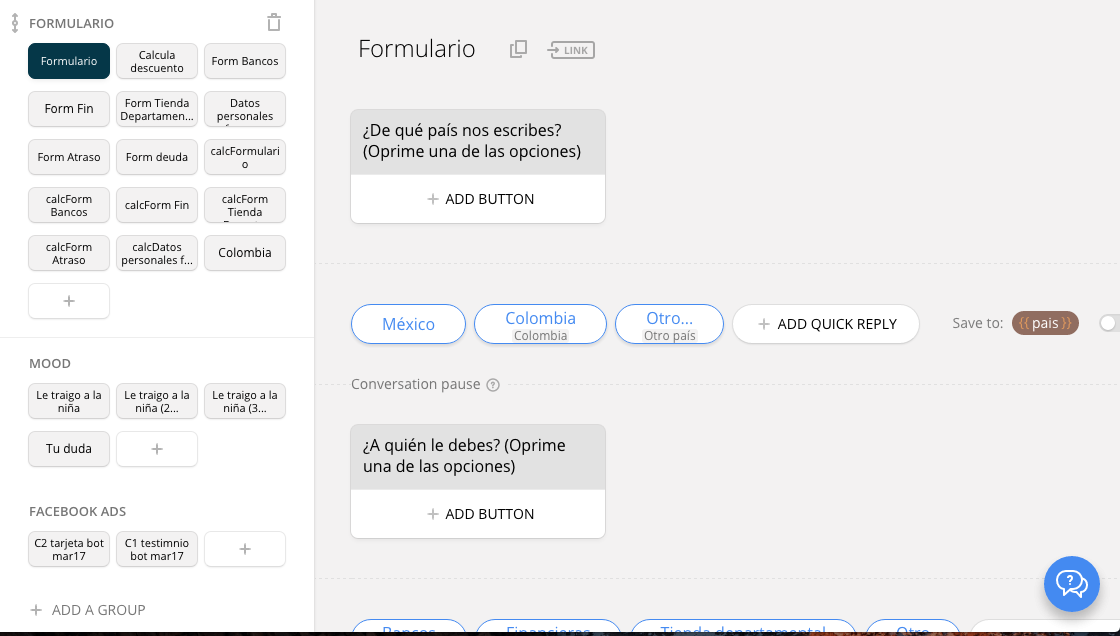
\includegraphics[width=\textwidth]{chatfuelFormulario.jpg}

\textbf{Cálculo de descuento, Formulario y Anuncios de Facebook}
Chatfuel funciona en este proyecto como el lugar para almacenar y crear la estructura del sistema que se presenta al usuario. Sin embargo, la funcionalidad requerida (hacer el cálculo de las cotizaciones, almacenar datos del usuario y datos de canales de adquisición de clientes) no es cubierta por la plataforma. Afortunadamente cuenta con conectores y APIs de integración a servicios externos. Por ello, se crearon integraciones y microservicios para las secciones de cálculo de descuento, formulario y anuncios de Facebook
\textbf{Flujo de cálculo de descuento y almacenamiento de datos}
Para hacer el cálculo del descuento se tenían que resolver dos cosas que no se pueden hacer directamente en Chatfuel. Hacer cálculos sobre datos insertados y almacenar datos en una base de datos. Por ello, se crearon dos micro servicios \textit{Lambda} \cite{kiran2015lambda}, \textbf{calculaDescuento} y \textbf{almacenaLeads}. Los cuales solucionan los dos aspectos faltantes de la herramienta.
Para acceder al micro servicio de \textbf{calculaDescuento} se utiliza un request GET con un query string que incluye los datos necesarios para el cálculo del descuento: deuda, banco, atraso de pago y si la persona ha pedido dejar sus datos ya. 
El servicio lo procesa y devuelve un mensaje con los datos insertados para el cálculo y el descuento resultante. Si el usuario aún no pide dejar sus datos se le invita a insertarlos para que un vendedor lo pueda contactar. 
El micro servicio \textbf{almacenaLeads} manda a través de un request POST los datos de contacto del usuario a la Base de datos: nombre completo, deuda, institución acreedora, atraso, e-mail, teléfono, campaña. Este servicio no genera ninguna respuesta al usuario.

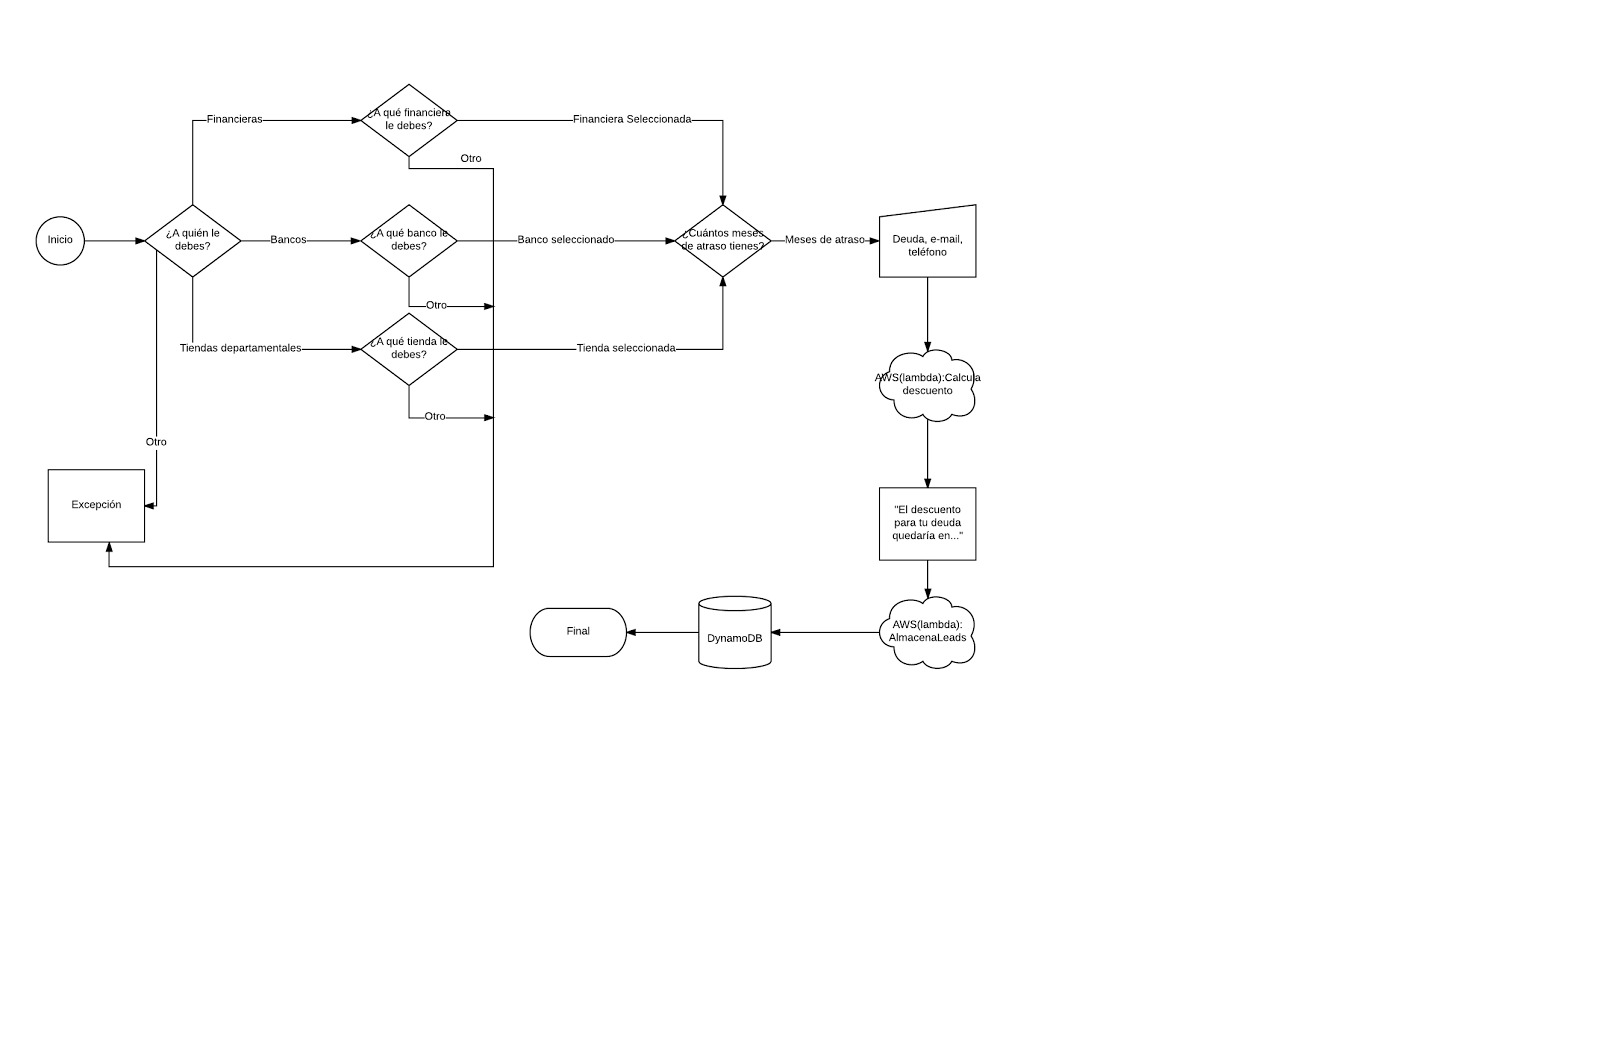
\includegraphics[width=\textwidth]{diagramaFlujoDatos.jpg}

\textbf{calculaDescuento}
La función recibe los datos que el bot le manda del usuario. Calcula el descuento a partir de la institución y meses que debe la persona. Estos valores fueron sacados de la forma en que se calcula el descuento en la página web promocional de Resuelve Tu Deuda; los cuales están basados en los promedios de los descuentos conseguidos por institución y meses de atraso.  Ese descuento se aplica a la deuda insertada y se calcula el monto final a pagar. Al final se regresa un objeto JSON con un mensaje indicando la deuda inicial, los meses de atraso, el porcentaje de descuento y el monto final estimado de su deuda si se hace cliente.
\textbf{almacenaLeads}
Para hacer la inserción al CRM, donde los vendedores ven los leads, se manda un POST a un endpoint que recibe los datos necesarios para hacer un registro nuevo (Nombre, teléfono, correo electrónico, meses de atraso, banco, system\_id, medio de contacto). Adicionalmente se añade una llave que asegura que el POST viene del bot.
\begin{itemize}
\item Se hacen un par de validaciones para verificar que los datos insertados sean válidos:
\item Se verifica que el correo tenga una terminación correcta de dominio (.com, .mx, etc) sino, se le añade ‘.com’ por default. Se verifica que ahora el formato sea correcto.
\item Se cambian todos los valores utf-8 a formato ascii
\item Se eliminan las comas presentes en los montos de deuda
\item Se transforma en un JSON
\item Y finalmente se envía a una función lambda que manda a Salesforce los nuevos leads.
\end{itemize}
El código detallado se encuentra en el apéndice

\textbf{Facebook Ads}
Una de la vía por la que más gente descubre a Resuelve es a través de los anuncios de Facebook. Por lo que se aprovechó esa ventaja para atraer gente a iniciar la conversación por esa vía también. Sin embargo, estos anuncios son pagados y deben ser monitoreados para que los costos por lead estén en los rangos esperados, así como el detalle de cual campaña tiene un mejor desempeño. Para solucionar esto se utilizó la estructura del objeto en JSON del mensaje mostrado al darle click a un anuncio que llevaba a Messenger. 
En la estructura del objeto JSON se utilizó la notación que utiliza Chatfuel para identificar los bloques que se deben mostrar y se asignó a cada anuncio un bloque de contenido. El cual consiste en una tarjeta que guarda en una variable el nombre de la campaña y redirige al usuario al mensaje de bienvenida (Figura 8). Para el usuario es un proceso transparente, sin embargo, el dato de la campaña se guarda en la base de datos si el usuario elige dejar sus datos de contacto.\cite{friedrich} 

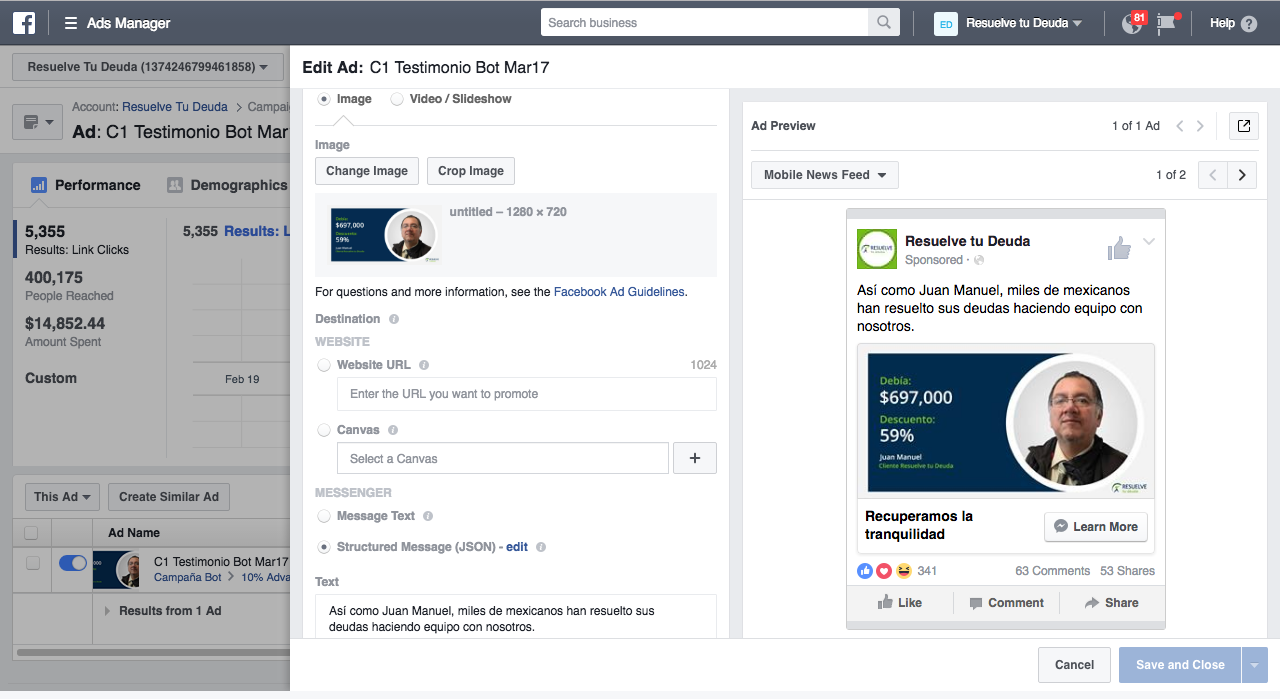
\includegraphics[width=\textwidth]{facebookAdsJSON.jpg}

\textbf{Procesamiento de Lenguaje Natural}
Los usuarios pueden conversar también a través de la introducción de frases con su teclado. Estas frases son interpretadas por el sistema de “AI” de Chatfuel, en donde se permite poner reglas, ejemplos de datos de entrada que armarán el modelo de procesamiento de lenguaje natural y la respuesta correcta como bloque de contenido o una respuesta corta de texto. Todo este procesamiento se hace con ayuda del algoritmo propietario de chatfuel.

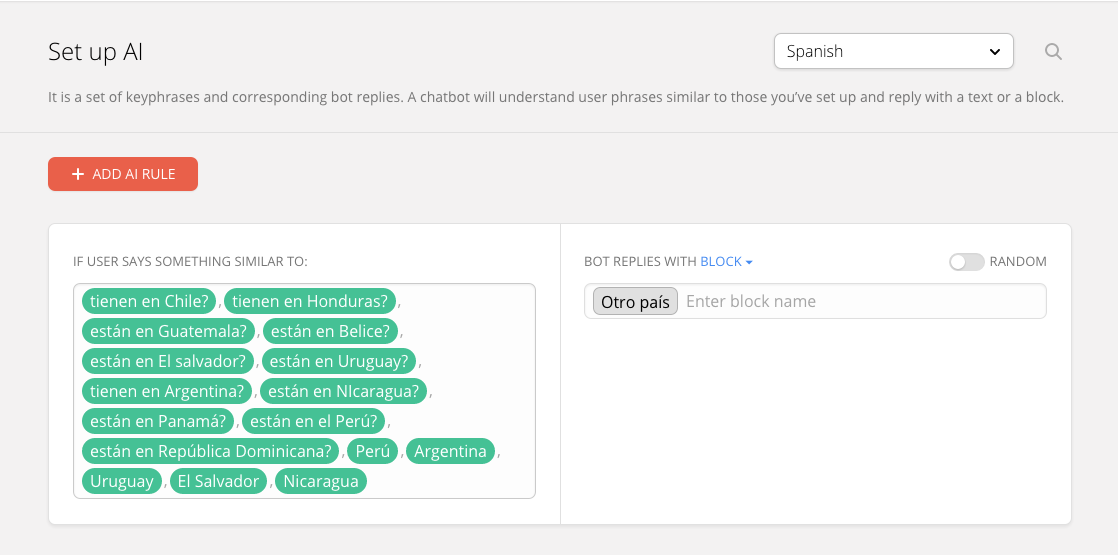
\includegraphics[width=\textwidth]{chatfuelAI.jpg}

Chatfuel recibe una consulta como datos de entrada. Con los datos trata de interpretar la consulta con la intención más adecuada en función de la información contenida (ejemplos, entidades utilizadas para anotaciones, contextos, parámetros, eventos) y el modelo de aprendizaje automático del agente, en este caso las reglas del chatbot. El algoritmo transforma el texto de la consulta en datos ejecutables y devuelve datos de salida como un objeto de respuesta JSON.

